\documentclass{beamer}
\usepackage[T1]{fontenc}
\usepackage[utf8]{inputenc}
\usepackage{lmodern}
\usepackage{graphicx}
\usepackage[brazil]{babel}
\usepackage[labelformat=empty]{caption}
\usetheme{JuanLesPins}

\title{
  \textbf{Design Sprint - Lighting Talks} \\
  CCSL - IME - USP
}

\begin{document}
\maketitle

\section{Introdução}

\begin{frame}
  \frametitle{Design Sprint}
  \framesubtitle{Conceito}

  \begin{itemize}
    \item O sprint é um processo para fornecer respostas às questões críticas de negócio
      \begin{itemize}
        \item Design
          \vspace{.25cm}
        \item Prototipagem
          \vspace{.25cm}
        \item Testando ideias com usuários
      \end{itemize}
      \vspace{.5cm}
    \item Desenvolvido pela Google Ventures
  \end{itemize}
\end{frame}

\begin{frame}
  \frametitle{Design Sprint}
  \framesubtitle{Etapas}
  \begin{figure}
    \begin{center}
      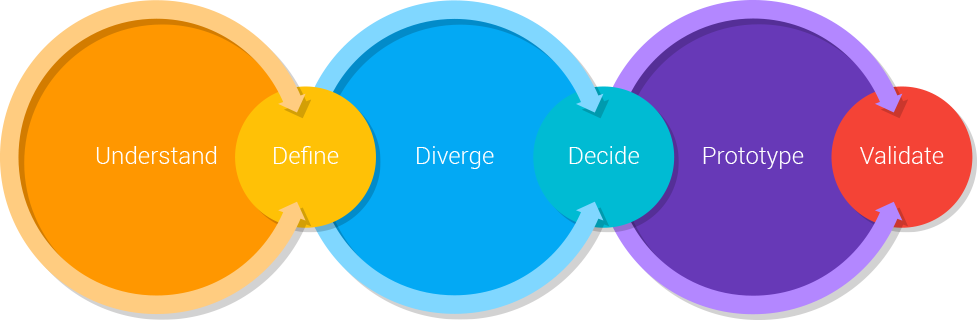
\includegraphics[width=\textwidth]{home-DS-flow-ill.png}\\
      \textbf{Ciclo Design Sprint}
    \end{center}
  \end{figure}
\end{frame}

\section{Mezuro}
\begin{frame}
  \frametitle{Mezuro}
  \framesubtitle{Motivação}
  \begin{itemize}
    \item Existem códigos bons e ruins
      \begin{itemize}
        \item Subjetivo
          \vspace{.25cm}
        \item Sem consenso
      \end{itemize}
      \vspace{.5cm}
    \item Critérios para avaliação podem ser extraídos
      \begin{itemize}
        \item Linhas de Código
          \vspace{.25cm}
        \item Quantidade de métodos
          \vspace{.25cm}
        \item Acoplamento
      \end{itemize}
      \vspace{.5cm}
    \item Já existem ferramentas para coleta dos critérios
  \end{itemize}
\end{frame}

\begin{frame}
  \frametitle{Mezuro}
  \framesubtitle{Motivação}

  Por que o uso de ferramentas não é difundido?

  \begin{itemize}
    \item Diferentes interfaces de interação
      \vspace{.5cm}
    \item Consomem tempo de processamento significativo
      \vspace{.5cm}
    \item Falta de interpretação sobre resultados
  \end{itemize}
\end{frame}

\begin{frame}
  \frametitle{Mezuro}
  \framesubtitle{}

  \begin{itemize}
    \item Diversas ferramentas em uma interface unificada
      \vspace{.25cm}
    \item Já provê interpretações padrão
      \vspace{.25cm}
    \item Permite configurações personalizadas
      \vspace{.25cm}
    \item Executa o processamento em segundo plano
      \vspace{.25cm}
    \item Inicia novos processamentos periodicamente
  \end{itemize}
\end{frame}

\section{Desafios}
\begin{frame}
  \frametitle{Fluxo de recuperação de senha}
  \framesubtitle{}

  \begin{itemize}
    \item Faltam informações ao usuário
      \vspace{.5cm}
    \item Links desnecessários
  \end{itemize}
\end{frame}

\begin{frame}
  \frametitle{Usabilidade na criação de configurações}
  \framesubtitle{}

  \begin{itemize}
    \item Estrutura complexa
      \vspace{.5cm}
    \item O caminho para realizar as tarefas não é intuitivo
      \vspace{.5cm}
    \item Funcionalidade para usuários avançados
  \end{itemize}
\end{frame}

\begin{frame}
  \frametitle{Exibição de estatísticas}
  \framesubtitle{}

  \begin{itemize}
    \item Temos dados sobre o uso de métricas
      \vspace{.5cm}
    \item Não exibimos essa informação em lugar algum
  \end{itemize}
\end{frame}

\begin{frame}
  \frametitle{Visualização das informações processadas}
  \framesubtitle{}

  \begin{itemize}
    \item Muita informação em uma única página
      \vspace{.5cm}
    \item Nomes ruins para seções
      \vspace{.5cm}
    \item Difícil entender a relação entre as partes
  \end{itemize}
\end{frame}

\end{document}
